\chapter{Le développement reproducteur et le contrôle de la floraison}\label{ch:b2:plant-flowering}

Un producteur de chrysanthèmes peut faire fleurir une serre pour Noël ou
pour Pâques en jouant sur l'éclairage~; un blé d'hiver semé au printemps
ne fleurit jamais, parce qu'il n'a pas eu froid~; une lampourde qui a
connu une seule nuit plus longue que sa durée critique est engagée dans
la floraison, quoi qu'il arrive ensuite. Une plante n'a pas de
calendrier, mais elle possède des horloges, des thermomètres et des
luxmètres, et elle décide une fois par an, sur leur témoignage, de
transformer un \omterm{def:b2:plant-meristems:meristem}{méristème} qui produisait des feuilles en un \omterm{def:b2:plant-meristems:meristem}{méristème} qui
produira une \omterm{def:b2:angiosperm-reproduction:flower}{fleur}. Ce chapitre suit cette décision depuis la feuille qui
mesure la nuit jusqu'au \omterm{def:b2:plant-meristems:meristem}{méristème} qui change de programme, puis la
construction de la \omterm{def:b2:angiosperm-reproduction:flower}{fleur} par un code de gènes, et la transition inverse
à l'autre bout du cycle~: la \omterm{def:b2:angiosperm-reproduction:seed}{graine} qui refuse de germer tant qu'on ne
lui a pas signalé que la saison est favorable.

\section{La transition florale}

\begin{definition}[Transition florale et induction]\label{def:b2:plant-flowering:transition}
\index{transition florale}\index{induction florale}\index{meristeme inflorescentiel@méristème inflorescentiel}
Un \omterm{def:b2:plant-meristems:meristem}{méristème apical caulinaire} végétatif produit indéfiniment des
feuilles portant chacune un bourgeon à leur aisselle. Lors de la
\emph{transition florale}, il devient un \emph{\omterm{def:b2:plant-meristems:meristem}{méristème}
inflorescentiel}, qui produit des bractées et, à leur aisselle, des
\emph{\omterm{def:b2:plant-meristems:meristem}{méristèmes} floraux}, chacun à croissance définie~: il produit
sépales, pétales, \omterm{def:b2:angiosperm-reproduction:flower}{étamines} et \omterm{def:b2:angiosperm-reproduction:flower}{carpelles}, puis s'arrête. Le changement
est déclenché par l'\emph{induction florale} --- un signal, venu des
feuilles ou issu de la physiologie propre de la plante, qui commute les
gènes d'identité du \omterm{def:b2:plant-meristems:meristem}{méristème}. Les plantes annuelles fleurissent une
fois et meurent~; les vivaces fleurissent chaque année à partir de
certains \omterm{def:b2:plant-meristems:meristem}{méristèmes} et en maintiennent d'autres à l'état végétatif. Le
moment de la floraison décide si le \omterm{def:b2:plant-life-cycles:heterospory}{pollen} rencontre le \omterm{def:b2:plant-life-cycles:heterospory}{pollen}, si les
\omterm{def:b2:angiosperm-reproduction:seed}{graines} mûrissent avant le gel, et si la \omterm{def:b2:angiosperm-reproduction:flower}{fleur} s'ouvre quand son
pollinisateur vole~: il est soumis à une forte sélection, et les plantes
ont acquis plusieurs manières de lire la saison.
\end{definition}

\begin{proposition}[Le photopériodisme~: la plante mesure la nuit]\label{prop:b2:plant-flowering:photoperiod}
\index{photoperiodisme@photopériodisme}\index{plante de jours courts}\index{plante de jours longs}\index{phytochrome}
De nombreuses plantes fleurissent en réponse à la durée du jour. Les
\emph{\omterm{prop:b2:plant-flowering:photoperiod}{plantes de jours courts}} (chrysanthème, soja, riz, lampourde)
fleurissent lorsque le jour est plus court qu'une durée critique --- en
automne ou au printemps~; les \emph{\omterm{prop:b2:plant-flowering:photoperiod}{plantes de jours longs}} (épinard,
blé, trèfle, \emph{Arabidopsis}) lorsqu'il est plus long --- au début
de l'été~; les plantes \emph{indifférentes} (tomate, maïs) fleurissent
lorsqu'elles sont assez grandes. Ce que mesure la plante est en réalité
la durée de la \emph{nuit} ininterrompue~: une \omterm{prop:b2:plant-flowering:photoperiod}{plante de jours courts} est
une plante de nuits longues, et un éclair de lumière au milieu d'une
longue nuit en annule l'effet, tandis qu'une période d'obscurité au
cours d'un long jour ne l'annule pas. La mesure est faite dans les
\emph{feuilles}, par le pigment \emph{phytochrome} --- une protéine qui
bascule entre une forme absorbant le rouge et une forme absorbant le
rouge lointain à chaque photon qu'elle capte, si bien que son état
enregistre la lumière --- confronté à une \emph{horloge circadienne}
interne d'environ vingt-quatre heures~: la floraison est déclenchée
lorsque la lumière coïncide avec une phase particulière de l'horloge,
ce qui ne se produit qu'à la bonne durée du jour.
\end{proposition}
\begin{proof}[Faits expérimentaux]
Garner et Allard (1920) constatèrent qu'un tabac mutant ne fleurissait
que dans les jours courts d'une serre d'hiver, et que des sojas semés à
intervalles réguliers tout l'été fleurissaient tous ensemble en
septembre~: c'était la durée du jour, et non l'âge ou la température,
qui fixait la date. Hamner et Bonner (1938) montrèrent chez la lampourde
qu'une seule nuit longue suffisait, qu'une minute de lumière au milieu
de la nuit supprimait l'effet, et que raccourcir le jour sans modifier
la nuit n'induisait pas la floraison. Borthwick et Hendricks (1952)
découvrirent que la lumière la plus efficace était rouge et qu'une
lumière rouge lointain donnée juste après le rouge l'annulait --- la
signature du phytochrome, isolé en 1959. La greffe d'une seule feuille
induite sur une plante non induite faisait fleurir la plante entière~:
la feuille exporte un signal.
\end{proof}

\begin{omfigure}
\begin{tikzpicture}[every node/.style={font=\scriptsize}]
  \foreach \y/\lab/\res in {3.6/{jour long, nuit courte}/{pas de fleur}, 2.7/{jour court, nuit longue}/{floraison}, 1.8/{nuit longue interrompue par un éclair}/{pas de fleur}, 0.9/{jour long interrompu par l'obscurité}/{pas de fleur}} {
    \node[anchor=east, align=right] at (-0.2,\y) {\lab};
    \node[anchor=west, omThm] at (8.6,\y) {\res};
  }
  % bars: 24 h = 8 cm; light yellow, dark grey
  \fill[omExo!30] (0,3.4) rectangle (8,3.8); \fill[yellow!50!orange!40] (0,3.4) rectangle (5.4,3.8);
  \fill[omExo!30] (0,2.5) rectangle (8,2.9); \fill[yellow!50!orange!40] (0,2.5) rectangle (3.0,2.9);
  \fill[omExo!30] (0,1.6) rectangle (8,2.0); \fill[yellow!50!orange!40] (0,1.6) rectangle (3.0,2.0); \fill[yellow!50!orange!40] (5.4,1.6) rectangle (5.55,2.0);
  \fill[omExo!30] (0,0.7) rectangle (8,1.1); \fill[yellow!50!orange!40] (0,0.7) rectangle (5.4,1.1); \fill[omExo!30] (2.6,0.7) rectangle (2.9,1.1);
  \draw[thick, ->] (0,0.3) -- (8.2,0.3); \foreach \x/\l in {0/0,2/6,4/12,6/18,8/24} \draw (\x,0.35) -- (\x,0.25) node[below] {\l};
  \node[below] at (4,-0.05) {heures};
  \draw[dashed, omDef] (5.4,0.3) -- (5.4,4.0); \node[omDef, above] at (5.4,4.0) {durée critique de la nuit};
\end{tikzpicture}

{\small La lampourde de Hamner et Bonner, une \omterm{prop:b2:plant-flowering:photoperiod}{plante de jours courts}.
Elle fleurit après une nuit plus longue que la durée critique~; une
minute de lumière au milieu de la nuit annule l'induction, tandis
qu'une période d'obscurité pendant le jour ne l'annule pas. La plante
mesure la nuit.}
\end{omfigure}

\begin{definition}[Le florigène]\label{def:b2:plant-flowering:florigen}
\index{florigene@florigène}\index{FLOWERING LOCUS T}
Le signal qu'exporte la feuille fut baptisé \emph{florigène} en 1937 et
identifié soixante-dix ans plus tard~: c'est une petite protéine, le
produit du gène \emph{FLOWERING LOCUS T} (FT). Dans la feuille,
l'horloge et le phytochrome n'activent ensemble FT que lorsque la durée
du jour convient (chez \emph{Arabidopsis}, \omterm{prop:b2:plant-flowering:photoperiod}{plante de jours longs},
lorsque la lumière coïncide avec le pic d'après-midi de l'activateur
CONSTANS, contrôlé par l'horloge)~; la protéine FT entre dans le phloème,
voyage avec le flux de sucres jusqu'à l'apex caulinaire et y active,
avec une protéine partenaire, les gènes qui transforment le \omterm{def:b2:plant-meristems:meristem}{méristème}.
La même protéine est le florigène du riz, \omterm{prop:b2:plant-flowering:photoperiod}{plante de jours courts}, chez
lequel l'horloge la câble en sens inverse. Les expériences de greffe, le
transport de la protéine dans le phloème et la floraison de plantes
chez lesquelles FT est exprimé sous le contrôle d'un promoteur propre
aux feuilles concordent~: la \omterm{def:b2:angiosperm-reproduction:flower}{fleur} se décide dans la feuille et
s'exécute dans le bourgeon.
\end{definition}

\begin{omfigure}
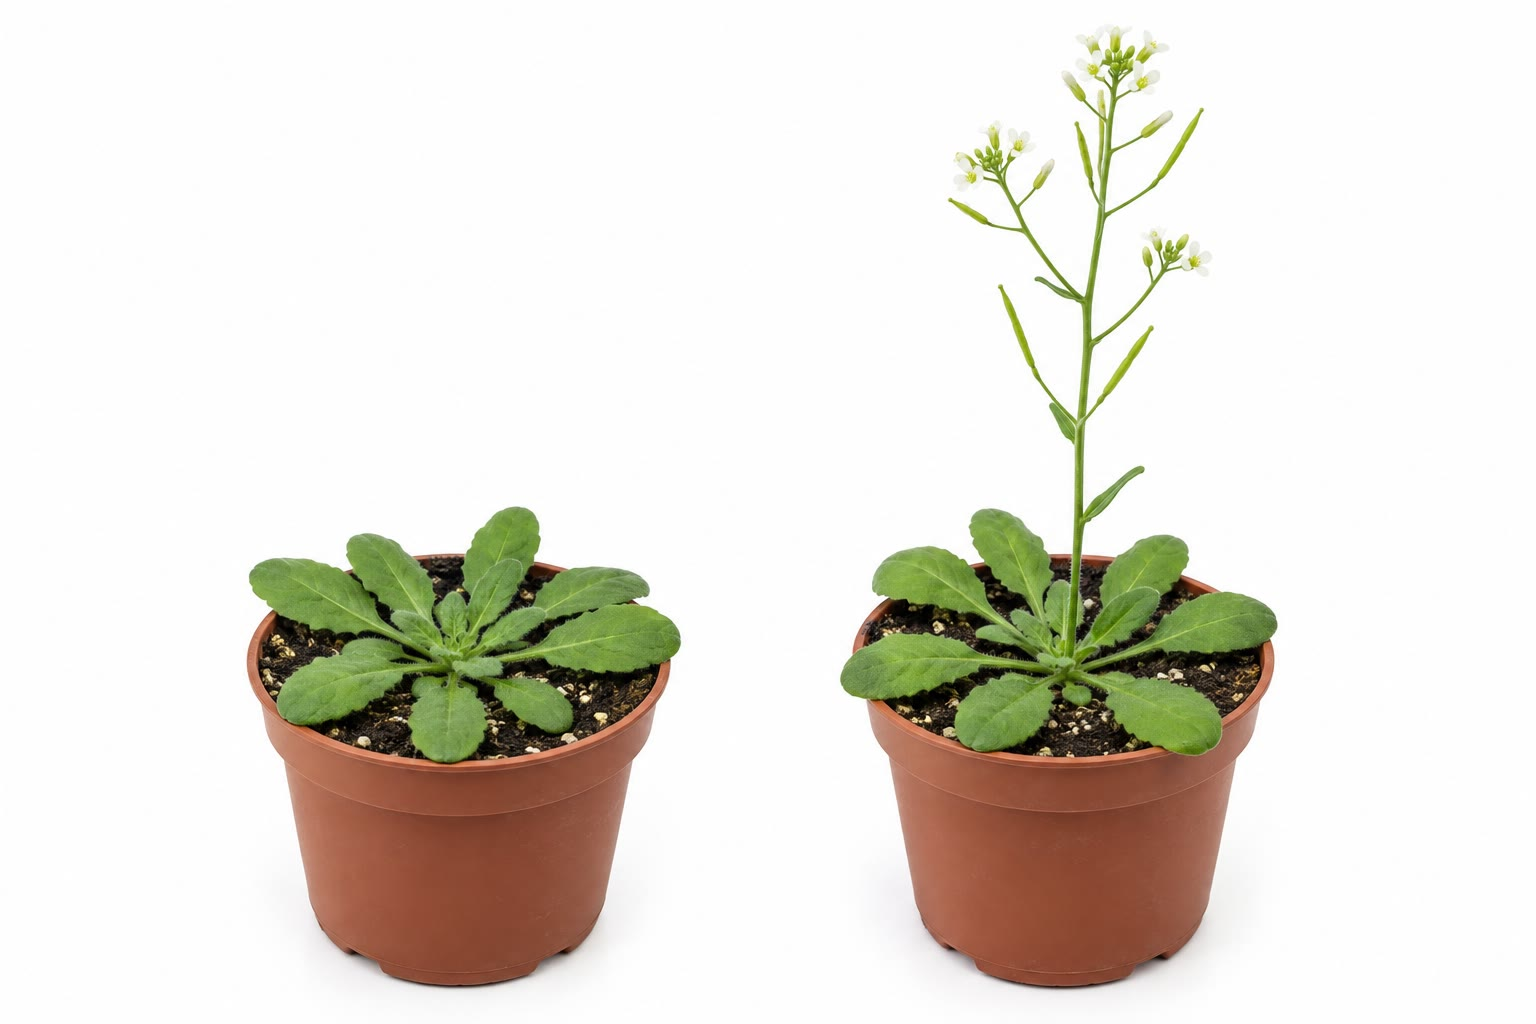
\includegraphics[width=0.58\linewidth]{images/book4/ai/b4-14-arabidopsis-daylength.jpg}

{\small \emph{Arabidopsis}, une \omterm{prop:b2:plant-flowering:photoperiod}{plante de jours longs}~: en jours courts,
une rosette de feuilles~; placée en jours longs, elle monte et fleurit
en quelques semaines.}
\end{omfigure}

\begin{proposition}[La vernalisation~: la plante compte le froid]\label{prop:b2:plant-flowering:vernalisation}
\index{vernalisation}\index{FLOWERING LOCUS C}
Les céréales d'hiver, les bisannuelles (carotte, chou, digitale) et de
nombreuses vivaces des climats froids ne fleurissent qu'après avoir
subi des semaines de froid --- la \emph{vernalisation} --- ce qui garantit
qu'une plante qui germe en automne attend le printemps au lieu de
fleurir en plein gel. Le froid est perçu par le \omterm{def:b2:plant-meristems:meristem}{méristème} lui-même, et
non par les feuilles~; aucun autre traitement ne peut le remplacer~; et
son effet est mémorisé pendant tout le reste de la croissance de la
plante, à travers des centaines de divisions cellulaires, mais pas à
travers la \omterm{def:b2:meiosis-heredity:meiosis}{méiose} --- toute \omterm{def:b2:angiosperm-reproduction:seed}{graine} repart non vernalisée. Chez
\emph{Arabidopsis}, la mémoire est un gène, \emph{\omterm{prop:b2:plant-flowering:vernalisation}{FLOWERING LOCUS C}}
(FLC), dont le produit réprime la floraison~: des semaines de froid le
réduisent progressivement au silence en recouvrant sa chromatine de
marques répressives, cette extinction est recopiée à chaque division,
et elle est effacée dans l'embryon. La plante \emph{intègre} ainsi le
froid au cours du temps --- quelques jours froids ne comptent pas --- et
un mutant dépourvu de FLC n'a besoin d'aucun hiver.
\end{proposition}

\begin{theorem}[Pourquoi l'intégration protège d'un faux printemps]\label{thm:b2:plant-flowering:integration}
Supposons qu'un répresseur soit réduit au silence à un taux constant
$\alpha$ par jour froid, si bien qu'après $n$ jours froids la fraction
encore active vaut $f_n = e^{-\alpha n}$, et que la floraison soit
permise lorsque $f < f_c$. Le nombre de jours froids nécessaires vaut
$n_c = \ln(1/f_c)/\alpha$, et --- comme l'extinction est stable --- les
jours froids n'ont pas besoin d'être consécutifs~: c'est leur total qui
compte. Une plante pour laquelle $n_c = 40$ jours n'est trompée ni par
un redoux de quinze jours en janvier ni par une vague de froid en
octobre~; une plante qui ne percevrait que la température du moment
fleurirait à la première semaine douce. La même intégration, assortie
d'un seuil, est la manière dont la plante lit la durée du jour
accumulée avant de s'engager~; ce sont deux exemples d'un système qui
répond à l'\emph{intégrale} d'un signal plutôt qu'à sa valeur
instantanée.
\end{theorem}
\begin{proof}
Si chaque jour froid réduit au silence une fraction $\alpha$ des copies
encore actives (ou de la chromatine encore non marquée), la fraction
active obéit à $f_{n+1} = (1 - \alpha)f_n \approx e^{-\alpha}f_n$,
d'où $f_n = e^{-\alpha n}$, $n$ étant le nombre de jours froids~;
l'inégalité $e^{-\alpha n} < f_c$ donne $n > \ln(1/f_c)/\alpha$. Les
jours qui ne sont pas froids n'ajoutent ni ne retranchent rien, puisque
les marques sont stables~: seul le total compte.
\end{proof}

\section{La construction de la fleur~: le modèle ABC}

\begin{proposition}[Le modèle ABC]\label{prop:b2:plant-flowering:abc}
\index{modele ABC@modèle ABC}\index{gene homeotique!floral@gène homéotique!floral}
Un \omterm{def:b2:plant-meristems:meristem}{méristème} floral met en place quatre verticilles concentriques~:
sépales, pétales, \omterm{def:b2:angiosperm-reproduction:flower}{étamines}, \omterm{def:b2:angiosperm-reproduction:flower}{carpelles}. Leurs identités sont fixées par
trois classes de \emph{gènes homéotiques}, qui agissent en anneaux
chevauchants~: la classe A seule, dans le verticille 1, donne des
sépales~; A et B ensemble, dans le verticille 2, des pétales~; B et C
ensemble, dans le verticille 3, des \omterm{def:b2:angiosperm-reproduction:flower}{étamines}~; C seule, dans le
verticille 4, des \omterm{def:b2:angiosperm-reproduction:flower}{carpelles}. A et C se répriment mutuellement, si bien
que là où l'une disparaît, l'autre s'étend à toute la \omterm{def:b2:angiosperm-reproduction:flower}{fleur}. Ces règles
prédisent chaque mutant simple~: sans B, la \omterm{def:b2:angiosperm-reproduction:flower}{fleur} est
sépale--sépale--carpelle--carpelle~; sans C, elle est
sépale--pétale--pétale--sépale, avec une autre \omterm{def:b2:angiosperm-reproduction:flower}{fleur} à l'intérieur,
puisque C arrête aussi le \omterm{def:b2:plant-meristems:meristem}{méristème}~; sans A, elle est
carpelle--étamine--étamine--carpelle. La plupart de ces gènes codent des
\omterm{prop:b2:cell-differentiation:transcriptional}{facteurs de transcription} d'une même famille (à boîte MADS), et une
quatrième classe, E, est nécessaire aux trois fonctions~; l'expression
conjointe de B et de C dans une feuille la transforme en un organe
semblable à une \omterm{def:b2:angiosperm-reproduction:flower}{étamine}. Les \omterm{def:b2:angiosperm-reproduction:flower}{fleurs} doubles des jardins --- roses,
pivoines, camélias --- sont des mutants de classe C, dont les \omterm{def:b2:angiosperm-reproduction:flower}{étamines}
sont devenues des pétales supplémentaires.
\end{proposition}
\begin{proof}[Faits expérimentaux]
Coen et Meyerowitz (1991) comparèrent les mutants homéotiques
d'\emph{Arabidopsis} et du muflier~: chez les deux, trois classes de
\omterm{def:b2:genome-diversification:mutation}{mutations} transformaient chacune deux verticilles adjacents, par les
mêmes paires, et les combinaisons de mutants se comportaient comme le
prévoit le modèle (le triple mutant ne produit que des feuilles). Le
clonage montra que ces gènes étaient des \omterm{prop:b2:cell-differentiation:transcriptional}{facteurs de transcription}
exprimés dans les anneaux prévus~; placer un gène B sous le contrôle d'un
promoteur actif dans les quatre verticilles donnait
pétale--pétale--étamine--étamine.
\end{proof}

\begin{omfigure}
\begin{tikzpicture}[every node/.style={font=\scriptsize}]
  % four whorls as columns
  \foreach \x/\w in {0/{verticille 1}, 2.2/{verticille 2}, 4.4/{verticille 3}, 6.6/{verticille 4}} \node[above] at (\x+0.9,3.3) {\w};
  \fill[omDef!35] (0,2.4) rectangle (4.2,3.1); \node at (2.1,2.75) {A};
  \fill[omProp!40] (2.2,1.6) rectangle (6.4,2.3); \node at (4.3,1.95) {B};
  \fill[omThm!30] (4.4,0.8) rectangle (8.6,1.5); \node at (6.5,1.15) {C};
  \foreach \x/\o in {0/sépales, 2.2/pétales, 4.4/étamines, 6.6/carpelles} \node[below, align=center] at (\x+0.9,0.6) {\o};
  \node[anchor=west, align=left] at (9.2,3.0) {type sauvage~: A, AB, BC, C};
  \node[anchor=west, align=left] at (9.2,2.3) {sans B~: sépale, sépale, carpelle, carpelle};
  \node[anchor=west, align=left] at (9.2,1.6) {sans C~: sépale, pétale, pétale, sépale\ldots};
  \node[anchor=west, align=left] at (9.2,0.9) {sans A~: carpelle, étamine, étamine, carpelle};
\end{tikzpicture}

{\small Le \omterm{prop:b2:plant-flowering:abc}{modèle ABC}. Trois classes de gènes disposées en anneaux
chevauchants fixent les quatre identités d'organes~; la perte d'une
classe transforme deux verticilles, et les \omterm{def:b2:angiosperm-reproduction:flower}{fleurs} mutantes sont
exactement celles que prévoit le modèle.}
\end{omfigure}

\begin{omfigure}
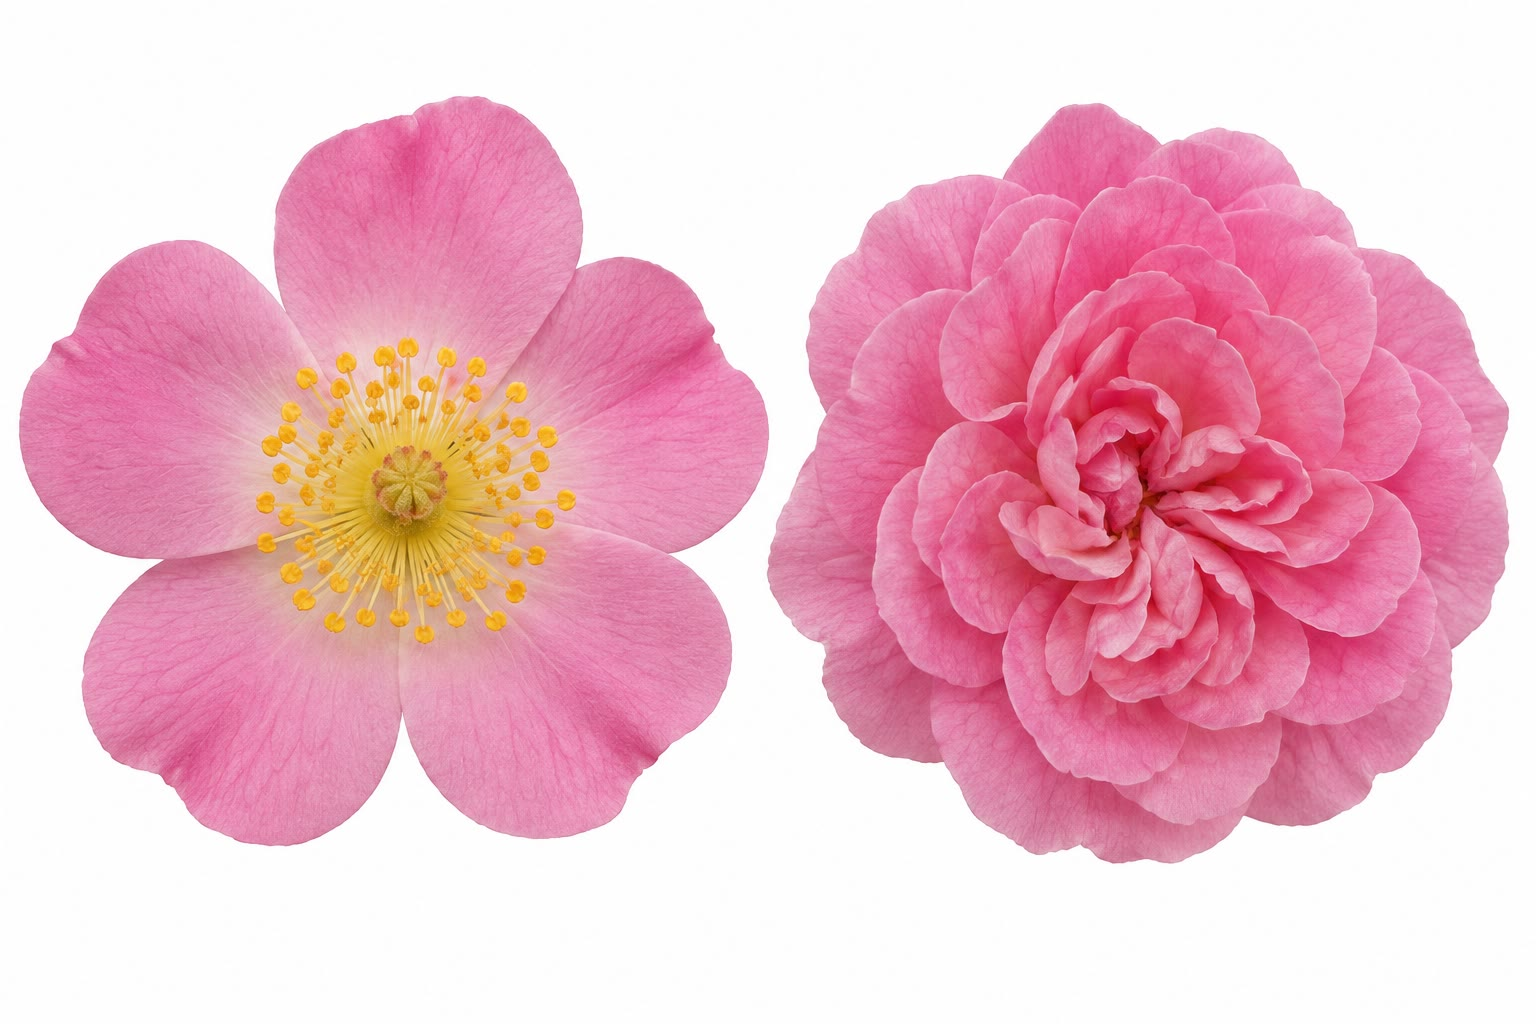
\includegraphics[width=0.58\linewidth]{images/book4/ai/b4-14-double-flower.jpg}

{\small Une \omterm{def:b2:angiosperm-reproduction:flower}{fleur} de type sauvage à côté d'une forme double~: les
\omterm{def:b2:angiosperm-reproduction:flower}{étamines} sont devenues des pétales --- un mutant de classe C, sélectionné
par les jardiniers pendant des siècles avant que quiconque ne sache
pourquoi la \omterm{def:b2:angiosperm-reproduction:flower}{fleur} était double.}
\end{omfigure}

\section{Dormance et germination}

\begin{definition}[La dormance des graines]\label{def:b2:plant-flowering:dormancy}
\index{dormance!des graines}\index{acide abscissique}\index{gibberelline@gibbérelline}\index{stratification}
Une \omterm{def:b2:angiosperm-reproduction:seed}{graine} viable qui ne germe pas dans des conditions qui
permettraient la croissance est \emph{dormante}. La \omterm{def:b2:angiosperm-reproduction:seed}{dormance} est
imposée pendant la maturation de la \omterm{def:b2:angiosperm-reproduction:seed}{graine} par l'\emph{acide
abscissique} (ABA), qui pilote aussi l'accumulation des réserves et la
dessiccation de l'embryon, et elle est maintenue par le tégument
(imperméable à l'eau ou au dioxygène, mécaniquement contraignant) ou par
l'état propre de l'embryon. Elle est levée par les signaux qui marquent
la fin de la saison défavorable~: des semaines de froid humide (la
\emph{stratification}, vernalisation de la \omterm{def:b2:angiosperm-reproduction:seed}{graine}), la lumière ---
pour les petites \omterm{def:b2:angiosperm-reproduction:seed}{graines} qui doivent se trouver près de la surface,
perçue par le phytochrome --- ou l'obscurité, l'alternance des
températures, le lessivage des inhibiteurs par la pluie, la
scarification du tégument par le sol ou par un tube digestif, la fumée
et la chaleur après un incendie. La décision résulte d'un équilibre
entre l'ABA et la \emph{gibbérelline}~: les signaux de levée abaissent
l'ABA et élèvent la gibbérelline, qui mobilise les réserves
(\cref{ch:b2:angiosperm-reproduction}) et permet à la radicule de
croître. Une population de \omterm{def:b2:angiosperm-reproduction:seed}{graines} n'est pas uniforme~: une fraction
germe à la première occasion, les autres attendent un an ou plus, si
bien qu'aucune mauvaise saison ne tue à elle seule toute la cohorte ---
c'est la \emph{banque de \omterm{def:b2:angiosperm-reproduction:seed}{graines}}, une assurance contre un monde
imprévisible.
\end{definition}
\begin{proof}[Faits expérimentaux]
Les \omterm{def:b2:angiosperm-reproduction:seed}{graines} de laitue (Borthwick, 1952) germent à l'obscurité après un
éclair de lumière rouge et non après un éclair de rouge lointain~;
soumises à rouge, puis rouge lointain, puis rouge, elles germent --- le
dernier éclair décide. Le même pigment réversible qui règle la
floraison déclenche la germination. Les \omterm{def:b2:angiosperm-reproduction:seed}{graines} de nombreux arbres
semées fraîches dans un sol chaud ne font rien~; les mêmes \omterm{def:b2:angiosperm-reproduction:seed}{graines}, après
deux mois dans un réfrigérateur humide, germent aussitôt, et des mutants
déficients en ABA germent sur la plante avant même que la \omterm{def:b2:angiosperm-reproduction:seed}{graine} soit
sèche.
\end{proof}

\begin{omfigure}
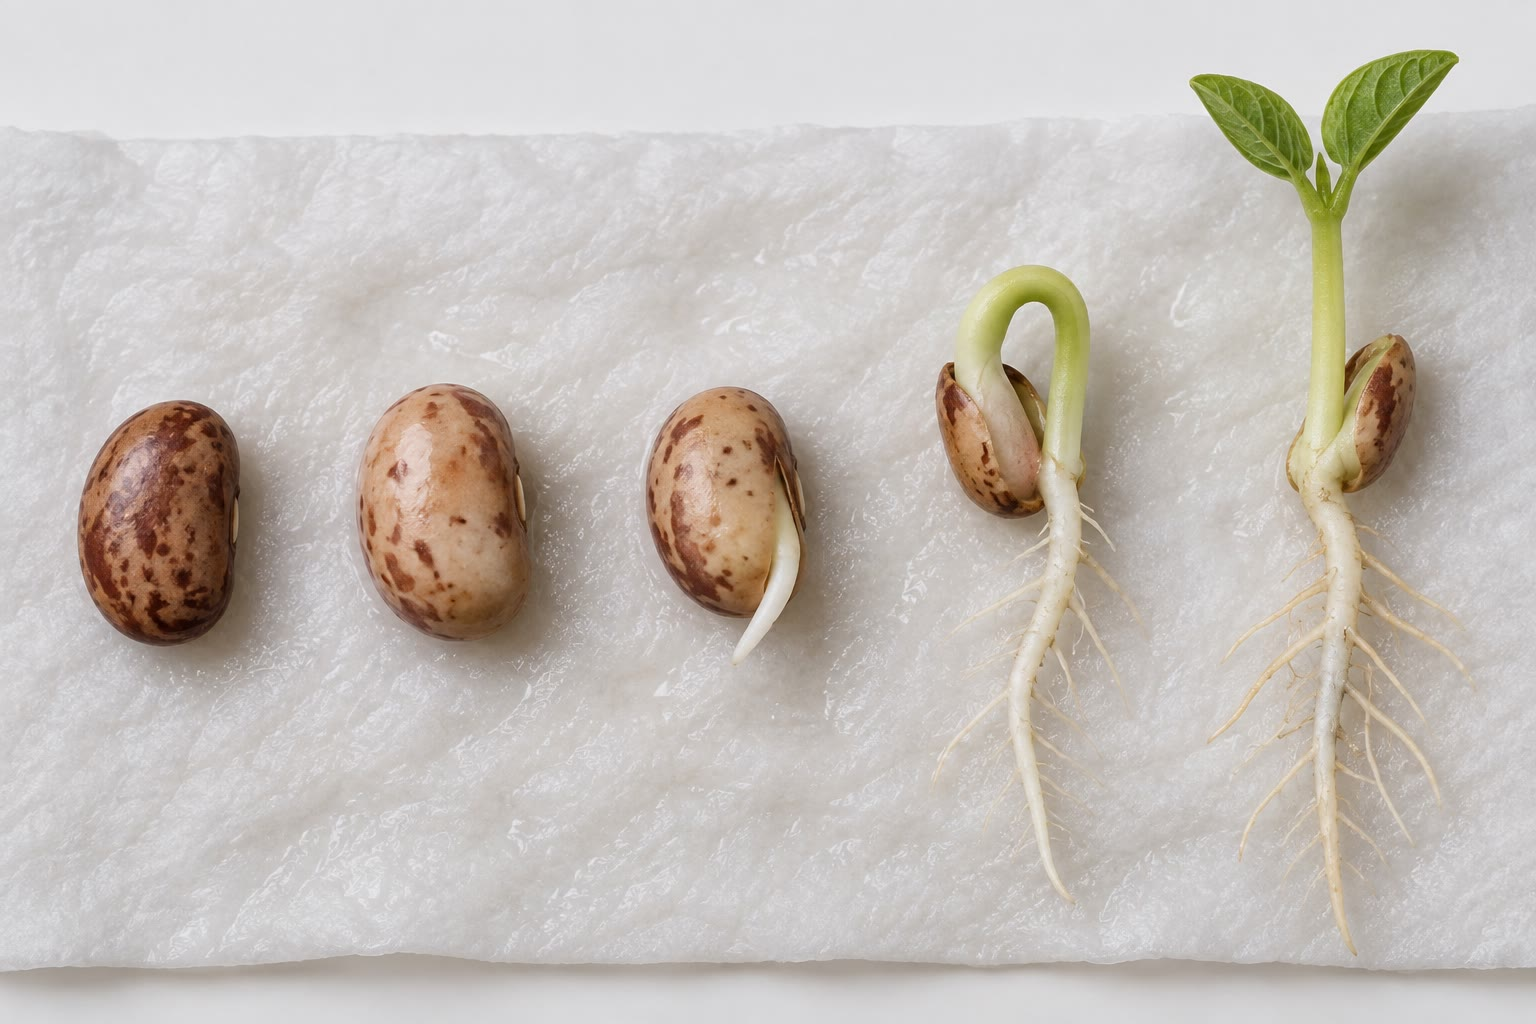
\includegraphics[width=0.66\linewidth]{images/book4/ai/b4-14-germinating-beans.jpg}

{\small La germination du haricot~: la \omterm{def:b2:angiosperm-reproduction:seed}{graine} s'imbibe, la radicule sort
la première, l'hypocotyle se recourbe en crochet pour traverser le sol,
et le crochet se redresse à la lumière à mesure que s'ouvrent les
premières feuilles.}
\end{omfigure}

\begin{theorem}[La germination comme pari]\label{thm:b2:plant-flowering:bet}
\index{diversification des risques}
Supposons qu'une fraction $g$ d'une cohorte de \omterm{def:b2:angiosperm-reproduction:seed}{graines} germe chaque
année et que le reste survive dans le sol jusqu'à l'année suivante avec
une probabilité $s$. Au cours d'une bonne année, une \omterm{def:b2:angiosperm-reproduction:seed}{graine} qui germe
laisse $R_g$ \omterm{def:b2:angiosperm-reproduction:seed}{graines}~; au cours d'une mauvaise année, aucune~; les années
sont bonnes avec une probabilité $p$. Une stratégie qui fait tout germer
d'un coup ($g = 1$) a, sur une suite d'années, un taux de croissance à
long terme, moyenné en $\ln$, égal à
$p\ln R_g + (1 - p)\ln 0 =
-\infty$~: une seule mauvaise année l'éteint. Une stratégie avec $g < 1$
croît pendant les bonnes années d'un facteur $gR_g + (1 - g)s$ et
pendant les mauvaises d'un facteur $(1 - g)s > 0$, si bien que son taux
à long terme,
\[
r = p\ln\bigl(gR_g + (1 - g)s\bigr) + (1 - p)\ln\bigl((1 - g)s\bigr),
\]
est fini et, pour $p$ pas trop proche de 1, maximal pour une valeur
intermédiaire de $g$. Avec $R_g = 20$, $s = 0.8$ et $p = 0.7$,
l'optimum se situe vers $g = 0.7$~: faire germer la plupart des \omterm{def:b2:angiosperm-reproduction:seed}{graines},
garder une réserve. La \omterm{def:b2:angiosperm-reproduction:seed}{dormance} n'est pas un échec de la germination,
mais un refus partiel sélectionné par l'évolution.
\end{theorem}
\begin{proof}
L'effectif au bout de $T$ années est le produit des facteurs annuels~;
son taux de croissance est donc la moyenne de leurs logarithmes (le taux
moyen géométrique), qui est ce que la sélection maximise sur de longues
périodes. Avec $g = 1$, le facteur des mauvaises années est nul et son
logarithme vaut $-\infty$. Pour $g < 1$, les deux facteurs sont
positifs~; dériver
$r$ par rapport à $g$ et annuler la dérivée donne l'optimum, qui, pour
les valeurs citées, se situe vers $g = 0.7$
(le calcul de $r$ pour $g = 0.4, 0.6, 0.8, 1$ donne $1.28$, $1.42$,
$1.40$, $-\infty$).
\end{proof}

\begin{omfigure}
\begin{tikzpicture}
\begin{axis}[
  width=0.7\linewidth, height=5.4cm,
  axis x line=bottom, axis y line=left,
  xmin=0, xmax=1, ymin=0, ymax=1.7,
  xlabel={fraction germant chaque année, $g$}, ylabel={taux de croissance à long terme $r$},
  xlabel style={font=\small, at={(axis description cs:0.5,-0.13)}, anchor=north},
  ylabel style={font=\small},
  tick label style={font=\small}, xtick={0,0.2,0.4,0.6,0.8,1}, ytick={0,0.5,1,1.5},
  clip=false,
]
\addplot[very thick, omDef, domain=0.02:0.97, samples=100] {0.7*ln(20*x + 0.8*(1-x)) + 0.3*ln(0.8*(1-x))};
\draw[dashed, gray] (axis cs:0.7,0) -- (axis cs:0.7,1.43);
\node[font=\scriptsize, anchor=south] at (axis cs:0.7,1.45) {optimum~: garder \qty{30}{\%} dans le sol};
\node[font=\scriptsize, anchor=north west, align=left] at (axis cs:0.7,0.6) {$g \to 1$~: une mauvaise année\\anéantit la cohorte};
\end{axis}
\end{tikzpicture}

{\small La \omterm{thm:b2:plant-flowering:bet}{diversification des risques} par la \omterm{def:b2:angiosperm-reproduction:seed}{dormance}. Avec sept bonnes
années sur dix, une cohorte qui germe entièrement finit par être
détruite par une mauvaise année~; une cohorte qui garde en réserve une
partie de ses \omterm{def:b2:angiosperm-reproduction:seed}{graines} croît le plus vite à long terme.}
\end{omfigure}

\section{Exercices}

\begin{exercise}[$\star$]\label{exo:b2:plant-flowering:1}
Distinguer \omterm{def:b2:plant-meristems:meristem}{méristèmes} végétatif, inflorescentiel et floral, et dire
lesquels sont à croissance définie.
\end{exercise}

\begin{exercise}[$\star$]\label{exo:b2:plant-flowering:2}
Définir \omterm{prop:b2:plant-flowering:photoperiod}{plantes de jours courts}, de jours longs et indifférentes, avec
un exemple de chacune, et dire ce que mesure réellement une \omterm{prop:b2:plant-flowering:photoperiod}{plante de
jours courts}.
\end{exercise}

\begin{exercise}[$\star$]\label{exo:b2:plant-flowering:3}
Donner l'identité des organes de chaque verticille chez le type sauvage
et chez les trois mutants simples du \omterm{prop:b2:plant-flowering:abc}{modèle ABC}.
\end{exercise}

\begin{exercise}[$\star$]\label{exo:b2:plant-flowering:4}
Nommer quatre signaux qui lèvent la \omterm{def:b2:angiosperm-reproduction:seed}{dormance} des \omterm{def:b2:angiosperm-reproduction:seed}{graines} et, pour
chacun, la saison ou le lieu qu'il signale.
\end{exercise}

\begin{exercise}[$\star\star$]\label{exo:b2:plant-flowering:5}
Une \omterm{prop:b2:plant-flowering:photoperiod}{plante de jours courts} a une nuit critique de \qty{10}{h}. Dire si
elle fleurit sous~: \qty{16}{h} de lumière/\qty{8}{h} d'obscurité~;
\qty{12}{h}/\qty{12}{h}~;
\qty{12}{h} de lumière, \qty{6}{h} d'obscurité, une minute de lumière,
\qty{6}{h} d'obscurité~;
\qty{8}{h} de lumière, \qty{4}{h} d'obscurité, \qty{4}{h} de lumière,
\qty{8}{h} d'obscurité.
\end{exercise}

\begin{exercise}[$\star\star$]\label{exo:b2:plant-flowering:6}
Une feuille d'une \omterm{prop:b2:plant-flowering:photoperiod}{plante de jours courts} induite est greffée sur une
\omterm{prop:b2:plant-flowering:photoperiod}{plante de jours longs} maintenue en jours longs, et la \omterm{prop:b2:plant-flowering:photoperiod}{plante de jours
longs} fleurit. Que montre ce résultat sur le \omterm{def:b2:plant-flowering:florigen}{florigène}~? Et si la
greffe est faite avec une feuille induite dont le phloème est
interrompu au niveau du pétiole~?
\end{exercise}

\begin{exercise}[$\star\star$]\label{exo:b2:plant-flowering:7}
Le froid réduit le répresseur au silence avec $\alpha = 0.05$ par jour,
et la floraison exige $f < 0.15$. Combien de jours froids faut-il~? Un
hiver comporte trois vagues de froid de 15, 12 et 20 jours séparées par
des redoux~: la plante est-elle vernalisée~? Et si $\alpha$ valait
$0.02$~?
\end{exercise}

\begin{exercise}[$\star\star$]\label{exo:b2:plant-flowering:8}
Expliquer, en termes de chromatine, pourquoi la mémoire d'une plante
vernalisée est perdue dans ses \omterm{def:b2:angiosperm-reproduction:seed}{graines}, et pourquoi c'est utile.
\end{exercise}

\begin{exercise}[$\star\star$]\label{exo:b2:plant-flowering:9}
Des \omterm{def:b2:angiosperm-reproduction:seed}{graines} de laitue reçoivent à l'obscurité les séquences~: R~; R puis
RL~; R, RL, R~; R, RL, R, RL. Prévoir la germination dans chaque cas et
l'expliquer à l'aide des deux formes du phytochrome.
\end{exercise}

\begin{exercise}[$\star\star\star$]\label{exo:b2:plant-flowering:10}
Dans le modèle de \omterm{thm:b2:plant-flowering:bet}{diversification des risques} avec $R_g = 20$,
$s = 0.8$, calculer le taux de croissance à long terme pour $g = 0.4$,
$0.6$, $0.8$ et $1$ lorsque
$p = 0.7$, puis lorsque $p = 0.95$. Comment l'optimum se déplace-t-il,
et que prédit-on pour les déserts par rapport aux prairies~?
\end{exercise}

\begin{exercise}[$\star\star\star$]\label{exo:b2:plant-flowering:11}
Prévoir la \omterm{def:b2:angiosperm-reproduction:flower}{fleur} obtenue en exprimant un gène de classe B dans les
quatre verticilles~; en exprimant la classe C dans les quatre~; chez un
double mutant dépourvu de A et de B. Expliquer ensuite pourquoi la \omterm{def:b2:angiosperm-reproduction:flower}{fleur}
sans C continue à former des verticilles.
\end{exercise}

\begin{exercise}[$\star\star\star$]\label{exo:b2:plant-flowering:12}
«~Une plante décide de fleurir en intégrant des signaux qu'elle ne
contrôle pas.~» Discuter les trois intégrations de ce chapitre --- de la
durée du jour, du froid, des années dans la banque de \omterm{def:b2:angiosperm-reproduction:seed}{graines} --- et ce
contre quoi un intégrateur protège la plante, qu'un simple seuil ne
protégerait pas.
\end{exercise}

\section{Problème~: le calendrier du producteur}

\begin{problem}[{Problème du week-end --- un producteur de chrysanthèmes
programme la floraison avec l'éclairage, un sélectionneur de blé compte
le froid, la fleur double d'un fleuriste est expliquée et la dormance
d'un lot de graines est modélisée, jusqu'à la durée de nuit qui
déclenche la culture, aux jours froids nécessaires au blé et à la
meilleure fraction de germination}]
\label{pb:b2:plant-flowering:1}
Le chrysanthème est une \omterm{prop:b2:plant-flowering:photoperiod}{plante de jours courts} dont la nuit critique
dure \qty{9.5}{h}~; l'induction exige \num{12} nuits inductives
consécutives, et les \omterm{def:b2:angiosperm-reproduction:flower}{fleurs} s'ouvrent \num{8} semaines après
l'induction. En novembre, la serre est dans l'obscurité de 17~h à
7~h~30. Le blé d'hiver a $\alpha = 0.06$ par jour froid et fleurit
lorsque $f < 0.10$. Lot de \omterm{def:b2:angiosperm-reproduction:seed}{graines}~: $R_g = 15$, $s = 0.7$, bonnes
années avec une probabilité $p$.

\medskip
\noindent\textbf{Partie I --- La serre.}
\begin{enumerate}
  \item En juin, la nuit naturelle dure \qty{8}{h}. La culture
        fleurira-t-elle~? Que doit faire le producteur pour vendre des
        \omterm{def:b2:angiosperm-reproduction:flower}{fleurs} en août~?
  \item Le producteur couvre la culture d'une toile noire de 19~h à
        7~h. Quelle durée de nuit la plante perçoit-elle, et quand le
        bâchage doit-il commencer pour une ouverture le 15~août~?
  \item En novembre, la nuit naturelle dure \qty{14}{h} et le producteur
        veut \emph{retarder} la floraison jusqu'à Noël. Proposer un
        programme d'éclairage et expliquer pourquoi un bref éclair
        suffit.
  \item L'éclair est donné à 21~h au lieu de minuit, et l'induction
        n'est pas empêchée. L'expliquer à l'aide de la durée critique de
        la nuit.
  \item Une nuit sur les douze, la toile n'est pas mise. Prévoir le
        résultat, et dire ce qu'aurait fait une lampourde.
  \item L'éclair donné en lumière verte échoue~; en lumière rouge, il
        réussit~; rouge suivi de rouge lointain échoue. Expliquer.
  \item Une seule feuille d'une plante induite est greffée sur une plante
        en jours longs. Prévoir le résultat, et dire ce qu'il identifie.
\end{enumerate}

\medskip
\noindent\textbf{Partie II --- Le blé.}
\begin{enumerate}[resume]
  \item De combien de jours froids le blé a-t-il besoin~?
  \item Semé en octobre, il reçoit 10 jours froids en novembre, un
        décembre doux, 25 en janvier et 12 en février. Quand est-il
        vernalisé~?
  \item Semé en mars, il reçoit 6 jours froids. Fleurit-il cet été-là~?
        Quelle en est la conséquence agricole~?
  \item Un mutant est dépourvu du répresseur. Prévoir son comportement et
        dire pourquoi les sélectionneurs appellent ces blés des «~blés de
        printemps~».
  \item Expliquer pourquoi la mémoire du froid survit aux divisions du
        \omterm{def:b2:plant-meristems:meristem}{méristème} au printemps mais pas à la \omterm{def:b2:meiosis-heredity:meiosis}{méiose} qui produit la
        génération suivante.
  \item Pourquoi le froid doit-il être compté dans le \omterm{def:b2:plant-meristems:meristem}{méristème} et non
        dans les feuilles, contrairement à la durée du jour~?
\end{enumerate}

\medskip
\noindent\textbf{Partie III --- Le fleuriste.}
\begin{enumerate}[resume]
  \item Une rose double a des pétales à la place des \omterm{def:b2:angiosperm-reproduction:flower}{étamines} et
        quelques pétales supplémentaires au centre. Quelle classe de
        gènes est défaillante~? Donner la formule des verticilles.
  \item De telles roses sont stériles comme parents pollinisateurs mais
        produisent parfois des \omterm{def:b2:angiosperm-reproduction:seed}{graines}. Expliquer ces deux faits à partir
        du \omterm{prop:b2:plant-flowering:abc}{modèle ABC}.
  \item Un muflier a des \omterm{def:b2:angiosperm-reproduction:flower}{étamines} à la place des pétales et des
        \omterm{def:b2:angiosperm-reproduction:flower}{carpelles} à la place des sépales. Quelle classe est défaillante~?
  \item Prévoir la \omterm{def:b2:angiosperm-reproduction:flower}{fleur} d'une plante chez laquelle la classe C est
        exprimée dans le verticille 1 en plus de ses verticilles
        normaux.
  \item Pourquoi les mêmes \omterm{def:b2:genome-diversification:mutation}{mutations} ont-elles produit les mêmes
        transformations chez une rose, un muflier et \emph{Arabidopsis},
        des plantes séparées par cent millions d'années~?
  \item Dans le verticille 2 d'une \omterm{def:b2:angiosperm-reproduction:flower}{fleur} de type sauvage, A et B sont
        tous deux actifs. Prévoir l'organe si seul B y était actif.
\end{enumerate}

\medskip
\noindent\textbf{Partie IV --- Le lot de \omterm{def:b2:angiosperm-reproduction:seed}{graines}.}
\begin{enumerate}[resume]
  \item Calculer le taux de croissance à long terme $r$ pour $g = 0.5$,
        $0.7$ et $0.9$ lorsque $p = 0.8$.
  \item Laquelle des trois valeurs est la meilleure~? Que se passe-t-il
        pour $g = 1$~?
  \item Refaire le calcul pour $p = 0.5$ (un désert). Quelle valeur de
        $g$ est la meilleure maintenant~?
  \item Un producteur sème tout le lot dans un seul champ au cours d'une
        bonne année et récolte $R_g$ \omterm{def:b2:angiosperm-reproduction:seed}{graines} par \omterm{def:b2:angiosperm-reproduction:seed}{graine}. Expliquer pourquoi
        sa stratégie diffère de celle de la plante et ce qu'il doit faire
        pour conserver la variété au-delà d'une mauvaise année.
  \item Les \omterm{def:b2:angiosperm-reproduction:seed}{graines} ont besoin de lumière pour germer. Expliquer l'intérêt
        adaptatif de ce trait pour une petite \omterm{def:b2:angiosperm-reproduction:seed}{graine}, et prévoir l'effet
        du labour sur la banque de \omterm{def:b2:angiosperm-reproduction:seed}{graines}.
  \item Énoncer le résultat~: la durée critique de la nuit et le
        programme de bâchage, le besoin en froid du blé, et la meilleure
        valeur de $g$ pour $p = 0.8$ et $p = 0.5$.
\end{enumerate}
\end{problem}
